%&"../ai"
\begin{document}
    \title{项目一:MSA}
    \maketitle
    % 1)对算法的描述以及算法实现结果分析;
    % 2)不同算法的搜索结果;
    % 3)不同算法的运行时间;
    % 4)复杂度分析。

    \tableofcontents
    \clearpage

    \section{题目}

    \subsection{Topic}

    Implement three algorithms to solve multiple sequence alignment (MSA) problems.

    \subsection{Requirements}

    \begin{enumerate}
        \item Implement dynamic programming (DP) algorithm to find the optimal solution.
        \item Implement A-star (A$^\ast$) algorithm to find the optimal solution.
        \item Implement genetic algorithm to find the optimal/suboptimal solution.
    \end{enumerate}

    \subsection{Rules}

    \begin{table}[H]
        \centering
        \caption{Cost Matrix}\label{tab:costmat}
        \begin{tabular}{cccc}
            \toprule
                & Match $\alpha(p,p)$ & Mismatch $\alpha(p,q)$ & Gap $\delta$ \\
            \midrule
            Cost & 0 & 3 & 2 \\
            \bottomrule
        \end{tabular}
    \end{table}

    The table above shows the pairwise cost matrix. For multiple sequence alignment, the cost should be calculated in a cycle pairwise manner. Note that GAP-GAP is a match and should be considered as 0 cost. For every query, find the best alignment(s) in the database with the lowest cost.

    \section{动态规划算法}

    在算法与复杂性课程\cite{algcom}里,已经提到了双序列比对的动态规划算法,如图 \ref{fig:pairwisedp} 所示,双序列比对对于一个状态只需要考虑三个临近状态的转移,分别是对齐$\alpha$,间隔 $\delta_x$、$\delta_y$,转换行动如表 \ref{tab:pairwise} 所示。对于每一个状态,都需要考虑经过哪一条路径消耗最小,于是就有了如算法 \ref{alg:pairwise} 的动态规划状态转移方程。

    \begin{algorithm}[H]
        \caption{双序列比对动态规划 MSA}\label{alg:pairwise}
        \KwIn{$x_1x_2\cdots x_m, y_1y_2\cdots y_n,\alpha,\delta$}
        \KwOut{}
        \BlankLine
        \lFor{$i\leftarrow 0$ to $m$}{$M[i,0]=i\delta$}
        \lFor{$j\leftarrow 0$ to $n$}{$M[0,j]=j\delta$}
        \For{$i\leftarrow 1$ to $m$}{
            \For{$j\leftarrow 1$ to $n$}{
                $M[i,j]=\min(\alpha[x_i,y_j] + M[i-1,j-1], \delta + M[i-1,j], \delta + M[i,j-1])$\;
            }
        }
        \Return{$M[m,n]$}\;
    \end{algorithm}

    \begin{minipage}{0.48\textwidth}
        \begin{table}[H]
            \centering
            \caption{双序列行动坐标变换表}\label{tab:pairwise}
            \begin{tabular}{crr}
                \toprule
                    & $i$ & $j$ \\
                \midrule
                $\alpha$ & $+1$ & $+1$ \\
                $\delta_x$ & $0$ & $+1$ \\
                $\delta_y$ & $+1$ & $0$ \\
                \bottomrule
            \end{tabular}
        \end{table}
    \end{minipage}\hfil
    \begin{minipage}{0.48\textwidth}
        \begin{figure}[H]
            \centering
            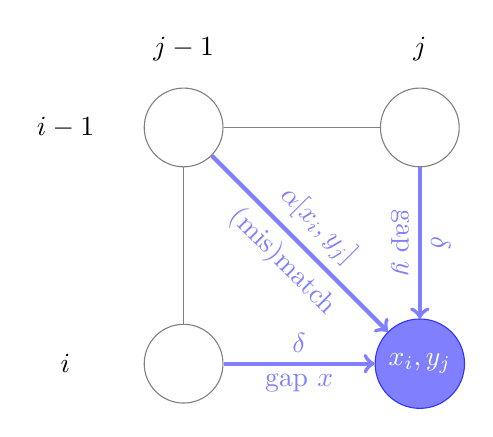
\begin{tikzpicture}
\tikzstyle{strnode}=[circle,draw=gray,minimum width=1cm];
\tikzstyle{move}=[line width=1.5pt, blue!50, ->];
\node[strnode] (v1) at (-1,0.5) {};
\node [strnode] (v3) at (2,0.5) {};
\node [strnode] (v4) at (-1,-2.5) {};
\node [strnode,fill=blue!50,draw=blue!80,font=\color{white}\bfseries] (v2) at (2,-2.5) {$x_i,y_j$};
\draw [move] (v1) edge node[sloped,above] {$\alpha[x_i,y_j]$} node[sloped,below] {(mis)match} (v2);
\draw [move] (v3) edge node[sloped,above] {$\delta$} node[sloped,below] {gap $y$} (v2);
\draw [move] (v4) edge node[sloped,above] {$\delta$} node[sloped,below] {gap $x$} (v2);
\draw[gray] (v1) edge (v3);
\draw[gray] (v1) edge (v4);
\node at (-2.5,0.5) {$i-1$};
\node at (-2.5,-2.5) {$i$};
\node at (2,1.5) {$j$};
\node at (-1,1.5) {$j-1$};
\end{tikzpicture}
            \caption{双序列比对}\label{fig:pairwisedp}
        \end{figure}
    \end{minipage}
    \medskip
    
    对于三序列比对,情况就复杂地多,需要同时考虑七条路径。

    \begin{minipage}{0.48\textwidth}
        \begin{table}[H]
            \centering
            \caption{三序列行动坐标变换表}\label{tab:multiple}
            \begin{tabular}{crrr}
                \toprule
                    & $i$ & $j$ & $k$ \\
                \midrule
                $\delta_x\delta_y\alpha_z$ & 0 & 0 & 1\\
                $\delta_x\alpha_y\delta_z$ & 0 & 1 & 0 \\
                $\delta_x\alpha_y\alpha_z$ & 0 & 1 & 1 \\
                $\alpha_x\delta_y\delta_z$ & 1 & 0 & 0 \\
                $\alpha_x\delta_y\alpha_z$ & 1 & 0 & 1 \\
                $\alpha_x\alpha_y\delta_z$ & 1 & 1 & 0 \\
                $\alpha_x\alpha_y\alpha_z$ & 1 & 1 & 1 \\
                \bottomrule
            \end{tabular}
        \end{table}
    \end{minipage}\hfil
    \begin{minipage}{0.48\textwidth}
        \begin{figure}[H]
            \centering
            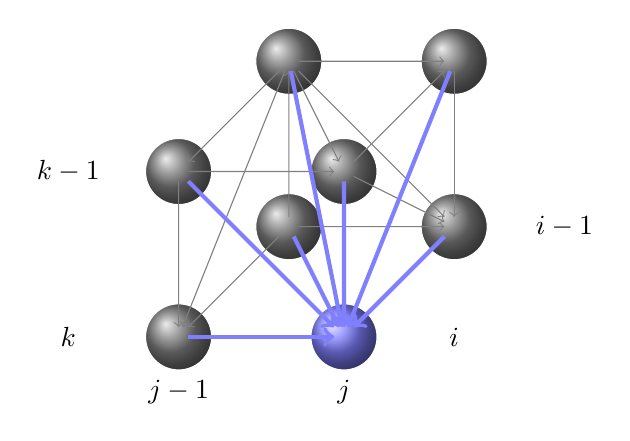
\begin{tikzpicture}[scale=1.4]
\tikzstyle{strnode}=[ball color=gray,white];
\tikzstyle{move}=[line width=1.5pt, blue!50, ->];
\tikzstyle{nomoce} = [gray, ->]
\draw[strnode] (-1.5,1.5) node (v1) {} circle (0.3cm);
\draw[strnode] (-1.5,3) node (v5) {} circle (0.3cm);
\draw[strnode] (0,3) node (v7) {} circle (0.3cm);
\draw[strnode] (0,1.5) node (v4) {} circle (0.3cm);
\draw[strnode, ball color=blue!50] (-1,0.5) node (v2) {} circle (0.3cm);
\draw[strnode] (-2.5,0.5) node (v3) {} circle (0.3cm);
\draw[strnode] (-2.5,2) node (v8) {} circle (0.3cm);
\draw[strnode] (-1,2) node (v6) {} circle (0.3cm);
\draw [nomoce] (v5) edge (v7);
\draw [nomoce] (v7) edge (v4);
\draw [nomoce] (v5) edge (v8);
\draw [nomoce] (v8) edge (v6);
\draw [nomoce] (v6) edge (v7);
\draw [nomoce] (v8) edge (v3);
\draw [nomoce] (v6) edge (v4);
\draw [nomoce] (v5) edge (v6);
\draw [nomoce] (v1) edge (v3);
\draw [nomoce] (v1) edge (v4);
\draw [nomoce] (v1) edge (v5);
\draw [nomoce] (v5) edge (v4);
\draw [nomoce] (v5) edge (v3);
\draw [move] (v1) edge (v2);
\draw [move] (v3) edge (v2);
\draw [move] (v4) edge (v2);
\draw [move] (v5) edge (v2);
\draw [move] (v6) edge (v2);
\draw [move] (v7) edge (v2);
\draw [move] (v8) edge (v2);
\node at (1,1.5) {$i-1$};
\node at (0,0.5) {$i$};
\node at (-1,0) {$j$};
\node at (-2.5,0) {$j-1$};
\node at (-3.5,0.5) {$k$};
\node at (-3.5,2) {$k-1$};
\end{tikzpicture}
            \caption{三序列比对}\label{fig:multipledp}
        \end{figure}
    \end{minipage}
    \medskip

    可以统一化为多序列比对问题。对于 $l$ 条序列比对,其行动转换方法可以被表示为二进制从 $(\underbrace{0\cdots01}_{l\text{ digits}})_2$ 到 $(\underbrace{1\cdots11}_{l\text{ digits}})_2$ 内所有的数,计算损耗使用上三角成对比较,规则统一为
    \begin{equation*}
        \texttt{compare}=
        \begin{cases}
            0,& (-,-) \| (p,p) \\
            2,& (p,-) \| (-,q) \\
            3,& (p,q)
        \end{cases}
    \end{equation*}
    并在确定每一次行动后记录路径,最后回溯路径到原点。

    % 29s

    \bibliography{ref}

\end{document}